% Options for packages loaded elsewhere
\PassOptionsToPackage{unicode}{hyperref}
\PassOptionsToPackage{hyphens}{url}
\PassOptionsToPackage{dvipsnames,svgnames,x11names}{xcolor}
\documentclass[
  spanish,
  11pt,
  a4paper,
]{article}
\usepackage{xcolor}
\usepackage[margin=23mm]{geometry}
\usepackage{amsmath,amssymb}
\setcounter{secnumdepth}{-\maxdimen} % remove section numbering
\usepackage{iftex}
\ifPDFTeX
  \usepackage[T1]{fontenc}
  \usepackage[utf8]{inputenc}
  \usepackage{textcomp} % provide euro and other symbols
\else % if luatex or xetex
  \usepackage{unicode-math} % this also loads fontspec
  \defaultfontfeatures{Scale=MatchLowercase}
  \defaultfontfeatures[\rmfamily]{Ligatures=TeX,Scale=1}
\fi
\usepackage{lmodern}
\ifPDFTeX\else
  % xetex/luatex font selection
\fi
% Use upquote if available, for straight quotes in verbatim environments
\IfFileExists{upquote.sty}{\usepackage{upquote}}{}
\IfFileExists{microtype.sty}{% use microtype if available
  \usepackage[]{microtype}
  \UseMicrotypeSet[protrusion]{basicmath} % disable protrusion for tt fonts
}{}
\makeatletter
\@ifundefined{KOMAClassName}{% if non-KOMA class
  \IfFileExists{parskip.sty}{%
    \usepackage{parskip}
  }{% else
    \setlength{\parindent}{0pt}
    \setlength{\parskip}{6pt plus 2pt minus 1pt}}
}{% if KOMA class
  \KOMAoptions{parskip=half}}
\makeatother
\usepackage{color}
\usepackage{fancyvrb}
\newcommand{\VerbBar}{|}
\newcommand{\VERB}{\Verb[commandchars=\\\{\}]}
\DefineVerbatimEnvironment{Highlighting}{Verbatim}{commandchars=\\\{\}}
% Add ',fontsize=\small' for more characters per line
\newenvironment{Shaded}{}{}
\newcommand{\AlertTok}[1]{\textcolor[rgb]{1.00,0.00,0.00}{\textbf{#1}}}
\newcommand{\AnnotationTok}[1]{\textcolor[rgb]{0.38,0.63,0.69}{\textbf{\textit{#1}}}}
\newcommand{\AttributeTok}[1]{\textcolor[rgb]{0.49,0.56,0.16}{#1}}
\newcommand{\BaseNTok}[1]{\textcolor[rgb]{0.25,0.63,0.44}{#1}}
\newcommand{\BuiltInTok}[1]{\textcolor[rgb]{0.00,0.50,0.00}{#1}}
\newcommand{\CharTok}[1]{\textcolor[rgb]{0.25,0.44,0.63}{#1}}
\newcommand{\CommentTok}[1]{\textcolor[rgb]{0.38,0.63,0.69}{\textit{#1}}}
\newcommand{\CommentVarTok}[1]{\textcolor[rgb]{0.38,0.63,0.69}{\textbf{\textit{#1}}}}
\newcommand{\ConstantTok}[1]{\textcolor[rgb]{0.53,0.00,0.00}{#1}}
\newcommand{\ControlFlowTok}[1]{\textcolor[rgb]{0.00,0.44,0.13}{\textbf{#1}}}
\newcommand{\DataTypeTok}[1]{\textcolor[rgb]{0.56,0.13,0.00}{#1}}
\newcommand{\DecValTok}[1]{\textcolor[rgb]{0.25,0.63,0.44}{#1}}
\newcommand{\DocumentationTok}[1]{\textcolor[rgb]{0.73,0.13,0.13}{\textit{#1}}}
\newcommand{\ErrorTok}[1]{\textcolor[rgb]{1.00,0.00,0.00}{\textbf{#1}}}
\newcommand{\ExtensionTok}[1]{#1}
\newcommand{\FloatTok}[1]{\textcolor[rgb]{0.25,0.63,0.44}{#1}}
\newcommand{\FunctionTok}[1]{\textcolor[rgb]{0.02,0.16,0.49}{#1}}
\newcommand{\ImportTok}[1]{\textcolor[rgb]{0.00,0.50,0.00}{\textbf{#1}}}
\newcommand{\InformationTok}[1]{\textcolor[rgb]{0.38,0.63,0.69}{\textbf{\textit{#1}}}}
\newcommand{\KeywordTok}[1]{\textcolor[rgb]{0.00,0.44,0.13}{\textbf{#1}}}
\newcommand{\NormalTok}[1]{#1}
\newcommand{\OperatorTok}[1]{\textcolor[rgb]{0.40,0.40,0.40}{#1}}
\newcommand{\OtherTok}[1]{\textcolor[rgb]{0.00,0.44,0.13}{#1}}
\newcommand{\PreprocessorTok}[1]{\textcolor[rgb]{0.74,0.48,0.00}{#1}}
\newcommand{\RegionMarkerTok}[1]{#1}
\newcommand{\SpecialCharTok}[1]{\textcolor[rgb]{0.25,0.44,0.63}{#1}}
\newcommand{\SpecialStringTok}[1]{\textcolor[rgb]{0.73,0.40,0.53}{#1}}
\newcommand{\StringTok}[1]{\textcolor[rgb]{0.25,0.44,0.63}{#1}}
\newcommand{\VariableTok}[1]{\textcolor[rgb]{0.10,0.09,0.49}{#1}}
\newcommand{\VerbatimStringTok}[1]{\textcolor[rgb]{0.25,0.44,0.63}{#1}}
\newcommand{\WarningTok}[1]{\textcolor[rgb]{0.38,0.63,0.69}{\textbf{\textit{#1}}}}
\usepackage{longtable,booktabs,array}
\usepackage{caption}
\captionsetup[table]{skip=6pt}
\newcounter{none} % for unnumbered tables
\usepackage{calc} % for calculating minipage widths
% Correct order of tables after \paragraph or \subparagraph
\usepackage{etoolbox}
\makeatletter
\patchcmd\longtable{\par}{\if@noskipsec\mbox{}\fi\par}{}{}
\makeatother
\usepackage{graphicx}
\makeatletter
\newsavebox\pandoc@box
\newcommand*\pandocbounded[1]{% scales image to fit in text height/width
  \sbox\pandoc@box{#1}%
  \Gscale@div\@tempa{\textheight}{\dimexpr\ht\pandoc@box+\dp\pandoc@box\relax}%
  \Gscale@div\@tempb{\linewidth}{\wd\pandoc@box}%
  \ifdim\@tempb\p@<\@tempa\p@\let\@tempa\@tempb\fi% select the smaller of both
  \ifdim\@tempa\p@<\p@\scalebox{\@tempa}{\usebox\pandoc@box}%
  \else\usebox{\pandoc@box}%
  \fi%
}
% Set default figure placement to htbp
\def\fps@figure{htbp}
\makeatother
\ifLuaTeX
\usepackage[bidi=basic,shorthands=off]{babel}
\else
\usepackage[bidi=default,shorthands=off]{babel}
\fi
\ifLuaTeX
  \usepackage{selnolig} % disable illegal ligatures
\fi
\setlength{\emergencystretch}{3em} % prevent overfull lines
\providecommand{\tightlist}{%
  \setlength{\itemsep}{0pt}\setlength{\parskip}{0pt}}
\usepackage{pdflscape}
\usepackage{etoolbox}
\AtBeginEnvironment{longtable}{\small}
\setlength{\tabcolsep}{5.5pt}
\setlength{\emergencystretch}{3em}
\setkeys{Gin}{keepaspectratio}
\usepackage{bookmark}
\IfFileExists{xurl.sty}{\usepackage{xurl}}{} % add URL line breaks if available
\urlstyle{same}
% fallback for those not using the hyperref driver hyperxmp:
\makeatletter
\@ifundefined{xmpquote}{\newcommand{\xmpquote}[1]{#1}}{}
\makeatother
\hypersetup{
  pdftitle={Tarea 3: Factorización LU distribuida con mpi4py},
  pdfauthor={José Ignacio Salas; Borja Smith; Josefina Abbott},
  pdflang={es},
  colorlinks=true,
  linkcolor={Maroon},
  filecolor={Maroon},
  citecolor={Blue},
  urlcolor={Blue},
  pdfcreator={LaTeX via pandoc}}

\title{Tarea 3: Factorización LU distribuida con mpi4py}
\usepackage{etoolbox}
\makeatletter
\providecommand{\subtitle}[1]{% add subtitle to \maketitle
  \apptocmd{\@title}{\par {\large #1 \par}}{}{}
}
\makeatother
\subtitle{IIC3533 · Computación de Alto Rendimiento · 2026-2}
\author{José Ignacio Salas \and Borja Smith \and Josefina Abbott}
\date{16 de noviembre de 2026}

\begin{document}
\maketitle

\section{Objetivo y metodología
experimental}\label{objetivo-y-metodologuxeda-experimental}

Se implementó y evaluó una factorización \(A=LU\) por bloques, sin
intercambio de filas, sobre un grid bidimensional de procesos MPI. La
matriz es densa, de doble precisión, con diagonal \(A_{ii}=N\) y
entradas restantes \(A_{ij}=\sin(10^{-3}ij+0.3i+0.7j)\). Su dominancia
diagonal permite trabajar sin pivoteo; además, el código verifica que
LAPACK no intercambie filas. Los factores se almacenan sobre el arreglo
original: \(U\) en el triángulo superior y la parte estrictamente
inferior de \(L\) bajo la diagonal; la diagonal unitaria de \(L\) es
implícita.

Se distingue entre el número de procesos MPI \(p=p_rp_c\), los threads
BLAS por proceso \(T\) y el número de CPUs utilizadas \(q=p_rp_cT\). El
tamaño de bloque es \(b\) y el número de bloques por dimensión es
\(n_b=N/b\); en los experimentos \(b\) divide a \(N\).

\subsection{Entornos utilizados}\label{entornos-utilizados}

La parte (a) se ejecutó en el MacBook Pro Apple M5 indicado en los
apuntes del grupo. El archivo de metadatos registra arquitectura arm64,
macOS 26.6.2, 10 CPUs lógicas, Python 3.11.18, NumPy 2.4.6, SciPy 1.17.1
y OpenBLAS 0.3.34. \texttt{threadpoolctl} confirmó un solo thread de
BLAS. La RAM no se registró en los metadatos y no se utiliza para
interpretar los resultados.

Los experimentos principales se realizaron en el cluster Kraken. Según
los apuntes de configuración, \texttt{ventress} dispone de dos sockets
Intel Xeon E5-2640 v4 y \texttt{yodaxico} de dos sockets Intel Xeon
Silver 4210R, ambos con 10 núcleos por socket y dos hilos de hardware
por núcleo. Se utilizó el entorno Conda del proyecto con mpi4py 4.1.2,
NumPy 2.4.6, SciPy 1.17.1 y Open MPI 5.0.11. Estas especificaciones y
versiones provienen de los registros del grupo, no de una nueva
ejecución de inventario.

Los jobs de un nodo se fijaron en \texttt{ventress}. Los de dos nodos
utilizaron \texttt{ventress} y \texttt{yodaxico}. SLURM reservó como
máximo 8 CPUs y 4 GB por nodo, con un límite de 15 minutos. Se usó
\texttt{-\/-threads-per-core=1} para asignar núcleos físicos distintos,
\texttt{-\/-cpus-per-task=T} y el lanzador \texttt{srun\ -\/-mpi=pmix}.
Las variables \texttt{OMP\_NUM\_THREADS},
\texttt{OPENBLAS\_NUM\_THREADS} y \texttt{MKL\_NUM\_THREADS} se fijaron
en \(T\) antes de importar NumPy. Así, los threads solicitados no
excedieron las CPUs reservadas por nodo.

\subsection{Medición y tratamiento de los
resultados}\label{mediciuxf3n-y-tratamiento-de-los-resultados}

Cada configuración tiene tres repeticiones. Se reporta la mediana y,
cuando corresponde, el mínimo y máximo observados. Estos extremos
describen la dispersión de la muestra; no son intervalos de confianza.
Los CSV originales se conservaron y las tablas del informe se calcularon
directamente a partir de ellos.

En serial se cronometra únicamente la factorización, excluyendo la
generación y copia inicial de la matriz. En distribuido cada proceso
sincroniza con \texttt{Barrier} antes del cronómetro y mide su tiempo de
pared \(t_{wall,r}\). El tiempo de ejecución es

\[t_{\max}=\max_{0\le r<p}t_{wall,r}.\]

El \texttt{Allreduce} que calcula este máximo, la construcción de la
matriz, la verificación y la escritura del CSV quedan fuera del
intervalo de factorización. Cada proceso acumula con
\texttt{MPI.Wtime()} dos mediciones:

\begin{itemize}
\tightlist
\item
  \(t_c\): factorización diagonal, resoluciones triangulares y
  actualización mediante producto matricial. La copia del bloque
  diagonal al buffer también está dentro de esta medición.
\item
  \(t_m\): tiempo dentro de los \texttt{Bcast}, incluyendo la espera
  hasta que los otros participantes estén listos.
\end{itemize}

Por tanto, \(t_m\) mide \textbf{comunicación y espera}, no transferencia
pura. Las asignaciones de buffers, las copias de paneles y el control de
Python no están todos incluidos en \(t_c+t_m\), aunque sí en
\(t_{wall}\). Las barras de cómputo/comunicación representan el promedio
entre procesos de una misma repetición: la que tiene el \(t_{\max}\)
mediano. No se suman máximos de procesos diferentes ni se confunde ese
promedio con el tiempo crítico.

El rendimiento se expresa como \(\mathrm{GFLOP/s}=(2N^3/3)/(10^9t)\),
usando el conteo dominante de operaciones de LU.

\section{(a) Tamaño de bloque en serial --- 10
puntos}\label{a-tamauxf1o-de-bloque-en-serial-10-puntos}

Se ejecutó \texttt{scripts/parte\_a.py} con \(N=4096\) y un thread BLAS.
Se probaron los bloques 4096, 2048, 1024, 512, 256, 128 y 64. Cada
repetición recorrió todos los bloques. La tabla procede de
\texttt{results/parte\_a\_mac\_jose.csv}.

{\def\LTcaptype{none} % do not increment counter
\begin{longtable}[]{@{}llllll@{}}
\toprule\noalign{}
\(b\) & \(N/b\) & Mediana {[}s{]} & Mín. {[}s{]} & Máx. {[}s{]} &
GFLOP/s \\
\midrule\noalign{}
\endhead
\bottomrule\noalign{}
\endlastfoot
4096 & 1 & 0.882 & 0.874 & 0.912 & 51.9 \\
2048 & 2 & 0.864 & 0.857 & 0.876 & 53.0 \\
1024 & 4 & 0.845 & 0.841 & 0.845 & 54.2 \\
512 & 8 & 0.853 & 0.851 & 0.856 & 53.7 \\
256 & 16 & 0.895 & 0.895 & 0.898 & 51.2 \\
128 & 32 & 0.984 & 0.980 & 1.021 & 46.5 \\
64 & 64 & 1.155 & 1.152 & 1.173 & 39.7 \\
\end{longtable}
}

Se elige \textbf{\(b=1024\)}, con mediana de 0.845 s y 54.2 GFLOP/s. Los
bloques 512 y 2048 quedaron aproximadamente a 1\% y 2\% del mejor
tiempo; es un mínimo relativamente plano para esta muestra. En cambio,
\(b=64\) demoró cerca de 37\% más.

El conteo dominante de operaciones no cambia con \(b\), pero sí su
reparto entre factorización diagonal, resoluciones triangulares y
productos matriciales. Bloques pequeños requieren más recorridos y
temporales y pueden aprovechar peor BLAS; bloques grandes concentran
trabajo en diagonal y paneles. El mínimo intermedio es compatible con
este compromiso. No se midieron contadores de caché para aislar sus
causas.

En los CSV, los residuos relativos están en el orden de \(10^{-16}\). El
checksum registrado es consistente entre bloques, pero la evidencia de
correctitud numérica es el residuo, no el checksum por sí solo.

\clearpage
\begin{landscape}

\begin{figure}
\centering
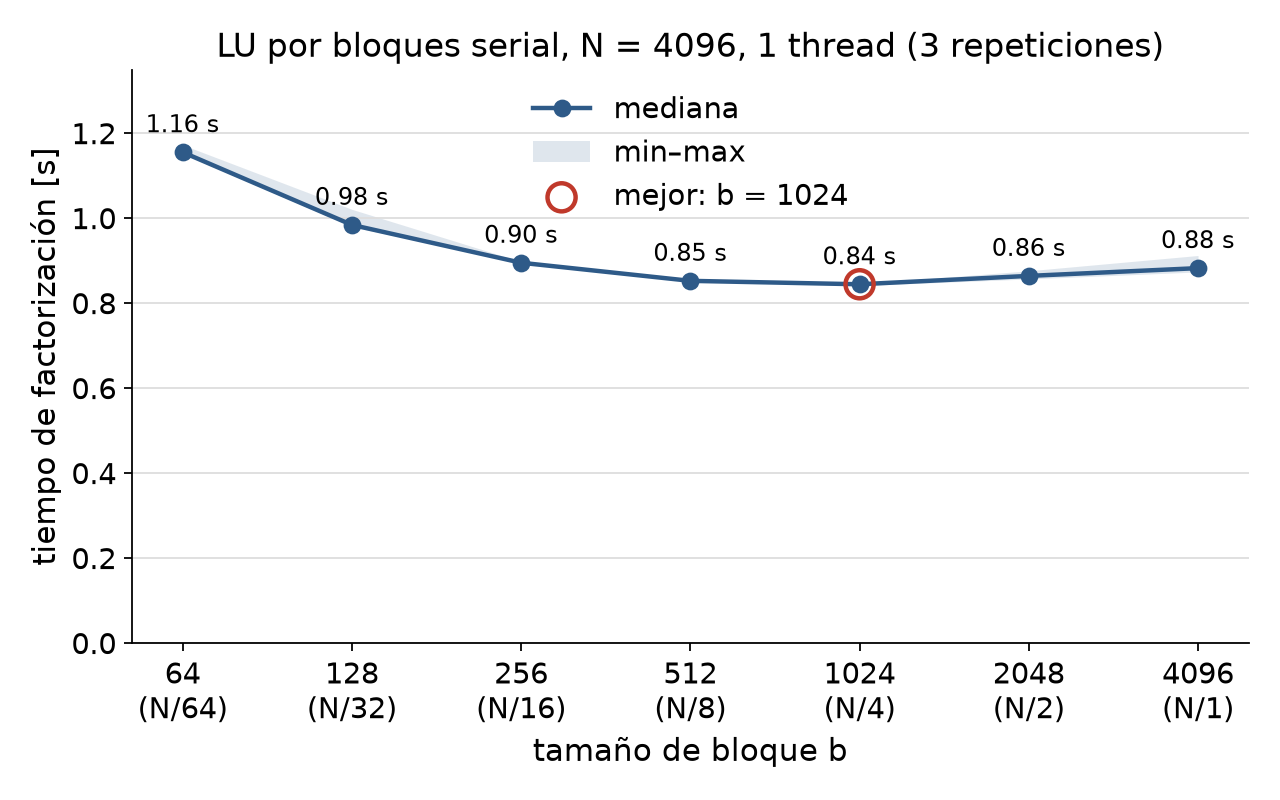
\includegraphics[width=240mm,height=155mm,alt={Barrido serial: mediana
de tres repeticiones y rango mínimo--máximo; N=4096, un
thread.}]{figuras/parte_a_mac_jose.png}
\caption{Barrido serial: mediana de tres repeticiones y rango
mínimo--máximo; N=4096, un thread.}
\end{figure}

\end{landscape}
\clearpage

\section{(b) Implementación distribuida --- 20
puntos}\label{b-implementaciuxf3n-distribuida-20-puntos}

\subsection{Distribución y almacenamiento
local}\label{distribuciuxf3n-y-almacenamiento-local}

\texttt{src/lu\_distributed.py} recibe \(N,b,p_r,p_c\) y exige
\(p_rp_c=\mathrm{size}\). El bloque global \(A_{IJ}\) pertenece al
proceso \((I\bmod p_r,J\bmod p_c)\). Cada proceso construye sus entradas
con \texttt{matrix\_entries} a partir de índices globales; así se
utiliza la misma matriz que en serial sin un \texttt{Scatter} inicial.

Los bloques de cada proceso se almacenan por índices globales crecientes
en un solo arreglo local de tamaño \((n_{lr}b)\times(n_{lc}b)\). En el
paso \(k\), sean \(i_s,j_s\) las cantidades de bloques locales de filas
y columnas con índice global menor o igual que \(k\). La parte aún no
factorizada corresponde a \texttt{Aloc{[}i\_s*b:,\ j\_s*b:{]}}; se
actualiza con \textbf{una sola multiplicación matricial por proceso y
paso}. Es una región rectangular del arreglo local, aunque la vista de
NumPy puede conservar un stride de fila mayor que su ancho y no ser
contigua en sentido C. Los paneles enviados se copian a buffers
contiguos.

La distribución también admite \(n_b\) no múltiplo de \(p_r\) o \(p_c\),
mediante tamaños locales distintos. En particular, no se presupone que
todos los procesos posean igual cantidad de bloques.

\subsection{Colectivas del paso
general}\label{colectivas-del-paso-general}

Se construyen \texttt{row\_comm\ =\ comm.Split(myrow,\ mycol)} y
\texttt{col\_comm\ =\ comm.Split(mycol,\ myrow)}. Dentro de
\texttt{row\_comm}, el rank local es \texttt{mycol}; dentro de
\texttt{col\_comm}, es \texttt{myrow}. En el paso \(k\) el dueño del
bloque diagonal es \((r,c)=(k\bmod p_r,k\bmod p_c)\).

{\def\LTcaptype{none} % do not increment counter
\begin{longtable}[]{@{}
  >{\raggedright\arraybackslash}p{(\linewidth - 6\tabcolsep) * \real{0.2500}}
  >{\raggedright\arraybackslash}p{(\linewidth - 6\tabcolsep) * \real{0.2500}}
  >{\raggedright\arraybackslash}p{(\linewidth - 6\tabcolsep) * \real{0.2500}}
  >{\raggedright\arraybackslash}p{(\linewidth - 6\tabcolsep) * \real{0.2500}}@{}}
\toprule\noalign{}
\begin{minipage}[b]{\linewidth}\raggedright
Difusión
\end{minipage} & \begin{minipage}[b]{\linewidth}\raggedright
Comunicador
\end{minipage} & \begin{minipage}[b]{\linewidth}\raggedright
Raíz local
\end{minipage} & \begin{minipage}[b]{\linewidth}\raggedright
Tamaño {[}float64{]}
\end{minipage} \\
\midrule\noalign{}
\endhead
\bottomrule\noalign{}
\endlastfoot
Bloque diagonal en fila \(r\) & \texttt{row\_comm} de esa fila & \(c\) &
\(b^2\) \\
Bloque diagonal en columna \(c\) & \texttt{col\_comm} de esa columna &
\(r\) & \(b^2\) \\
Panel \(L\) de cada fila del grid & \texttt{row\_comm} de cada fila &
\(c\) & \((n_{lr}-i_s)b^2\) \\
Panel \(U\) de cada columna del grid & \texttt{col\_comm} de cada
columna & \(r\) & \((n_{lc}-j_s)b^2\) \\
\end{longtable}
}

Primero, el dueño factoriza \(A_{kk}\) y difunde el bloque empaquetado
de \(L_{kk}\) y \(U_{kk}\) en su fila y columna. Solo los integrantes de
esos comunicadores participan en estas dos difusiones. Los procesos de
la fila \(r\) calculan \(U_{kj}=L_{kk}^{-1}A_{kj}\); los de la columna
\(c\) calculan \(L_{ik}=A_{ik}U_{kk}^{-1}\), implementado mediante una
resolución triangular transpuesta.

Después se difunden los paneles: en cada fila la raíz es el proceso de
columna \(c\), y en cada columna la raíz es el proceso de fila \(r\).
Todos participan en estas difusiones de sus respectivos comunicadores,
incluso si el panel tiene cero elementos. Finalmente cada proceso con
filas y columnas pendientes ejecuta
\(A_{local}\leftarrow A_{local}-L_{panel}U_{panel}\). La factorización
utiliza \texttt{Bcast}; \texttt{gather} aparece en la verificación y
recolección de resultados, fuera del núcleo medido.

Por ejemplo, para \(k=2\) y grid \(2\times3\), el dueño de \(A_{22}\) es
\((0,2)\). Este difunde por fila con raíz local 2 y por columna con raíz
local 0. El proceso \((1,1)\) recibe \([L_{32};L_{52}]\) desde \((1,2)\)
por su fila y \(U_{24}\) desde \((0,1)\) por su columna, y actualiza
conjuntamente \([A_{34};A_{54}]\) con un producto.

\subsection{Verificación y control de
recursos}\label{verificaciuxf3n-y-control-de-recursos}

Con \texttt{-\/-verify}, los bloques se reúnen en rank 0, se reconstruye
la matriz de factores y se ejecuta la versión serial sobre la misma
matriz y con el mismo \(b\). Se calculan

\[\delta=\frac{\max_{ij}|(LU_{dist}-LU_{serial})_{ij}|}{\max_{ij}|(LU_{serial})_{ij}|},\qquad
\rho=\frac{\|A-LU\|_F}{\|A\|_F}.\]

El programa exige que ambos sean menores que \(10^{-8}\). Según los
apuntes de verificación del grupo, los 12 casos locales de
\texttt{scripts/test\_distributed.sh} pasaron con \(\delta=0\) y
residuos aproximadamente entre \(1.6\times10^{-16}\) y
\(2.2\times10^{-16}\).

{\def\LTcaptype{none} % do not increment counter
\begin{longtable}[]{@{}
  >{\raggedright\arraybackslash}p{(\linewidth - 2\tabcolsep) * \real{0.5000}}
  >{\raggedright\arraybackslash}p{(\linewidth - 2\tabcolsep) * \real{0.5000}}@{}}
\toprule\noalign{}
\begin{minipage}[b]{\linewidth}\raggedright
Casos del script
\end{minipage} & \begin{minipage}[b]{\linewidth}\raggedright
Cobertura
\end{minipage} \\
\midrule\noalign{}
\endhead
\bottomrule\noalign{}
\endlastfoot
\(1\times1\), \(N=512,b=64\) & Equivalencia con serial \\
\(2\times2\), \(N=512,b=64,256,512\) & Bloques pequeños y caso
\(b=N\) \\
\(1\times4\) y \(4\times1\), \(N=512,b=64\) & Grids con una dimensión
unitaria \\
\(2\times3\), \(N=384,b=32\) & Distribución de 12 bloques por
dimensión \\
\(2\times3\) y \(3\times2\), \(N=640,b=64\) & \(n_b=10\), no múltiplo de
todas las dimensiones \\
\(2\times4\), \(N=1024,b=128\); \(4\times2\), \(N=1024,b=64\) & Grids de
ocho procesos \\
\(2\times2\), \(N=1000,b=100\) & Tamaño no potencia de dos \\
\end{longtable}
}

Los apuntes del cluster también registran verificación correcta en dos
nodos, con diferencia relativa \(4.4\times10^{-16}\) y residuo
\(1.5\times10^{-16}\). Por ello no se afirma identidad bit a bit para
cualquier hardware: las diferencias de BLAS pueden cambiar el redondeo.
Estos resultados históricos se complementaron con una nueva revisión
local el 15 de noviembre: se ejecutaron los cinco tests de distribución
y los 14 casos de la suite ampliada, todos correctos. Los dos casos
adicionales (\(2\times3,N=64,b=64\) y \(1\times8,N=64,b=32\)) ejercitan
procesos sin bloques locales y paneles vacíos. En esta revisión las
diferencias frente a serial fueron cero y los residuos estuvieron entre
\(1.21\times10^{-16}\) y \(2.17\times10^{-16}\). Se conservaron las
salidas y el entorno en \texttt{informe/verificacion/}. Estas pruebas
pequeñas verifican correctitud; no sustituyen las mediciones de
rendimiento del cluster. El \texttt{gather} de verificación se reserva
para problemas pequeños y se excluye de las mediciones grandes.

Para evitar oversubscription se fija \(T\) antes de cargar BLAS y se
respeta \(pT\leq\) núcleos disponibles en la ejecución local, o la
asignación por nodo de SLURM en el cluster. En particular, grid
\(2\times2\) con \(T=2\) utiliza 8 CPUs; grid \(4\times4\) con \(T=1\)
utiliza 16 CPUs distribuidas en dos nodos.

\clearpage

\section{(c) Tamaño de bloque en el cluster --- 10
puntos}\label{c-tamauxf1o-de-bloque-en-el-cluster-10-puntos}

Se utilizó \(N=8192\), configuración 2, grid \(2\times2\), \(T=2\), un
nodo \texttt{ventress} y tres repeticiones por bloque. La fuente es
\texttt{results/cluster/parte\_c.csv}, job 37838. Se incluyen los
bloques de (a) y, adicionalmente, \(b=8192\) como caso extremo de un
único bloque.

{\def\LTcaptype{none} % do not increment counter
\begin{longtable}[]{@{}
  >{\raggedright\arraybackslash}p{(\linewidth - 12\tabcolsep) * \real{0.1429}}
  >{\raggedright\arraybackslash}p{(\linewidth - 12\tabcolsep) * \real{0.1429}}
  >{\raggedright\arraybackslash}p{(\linewidth - 12\tabcolsep) * \real{0.1429}}
  >{\raggedright\arraybackslash}p{(\linewidth - 12\tabcolsep) * \real{0.1429}}
  >{\raggedright\arraybackslash}p{(\linewidth - 12\tabcolsep) * \real{0.1429}}
  >{\raggedright\arraybackslash}p{(\linewidth - 12\tabcolsep) * \real{0.1429}}
  >{\raggedright\arraybackslash}p{(\linewidth - 12\tabcolsep) * \real{0.1429}}@{}}
\toprule\noalign{}
\begin{minipage}[b]{\linewidth}\raggedright
\(b\)
\end{minipage} & \begin{minipage}[b]{\linewidth}\raggedright
\(t_{\max}\) {[}s{]}
\end{minipage} & \begin{minipage}[b]{\linewidth}\raggedright
Mín. {[}s{]}
\end{minipage} & \begin{minipage}[b]{\linewidth}\raggedright
Máx. {[}s{]}
\end{minipage} & \begin{minipage}[b]{\linewidth}\raggedright
\(\bar t_c\) {[}s{]}
\end{minipage} & \begin{minipage}[b]{\linewidth}\raggedright
\(\bar t_m\) {[}s{]}
\end{minipage} & \begin{minipage}[b]{\linewidth}\raggedright
GFLOP/s
\end{minipage} \\
\midrule\noalign{}
\endhead
\bottomrule\noalign{}
\endlastfoot
8192 & 8.062 & 8.036 & 8.162 & 1.911 & 4.082 & 45.5 \\
4096 & 6.520 & 6.378 & 6.622 & 1.881 & 3.324 & 56.2 \\
2048 & 3.918 & 3.898 & 3.966 & 1.824 & 1.857 & 93.6 \\
1024 & 2.905 & 2.900 & 2.940 & 1.820 & 1.020 & 126.2 \\
512 & 2.589 & 2.587 & 2.625 & 1.924 & 0.630 & 141.6 \\
256 & 2.738 & 2.721 & 2.767 & 2.250 & 0.460 & 133.8 \\
128 & 3.464 & 3.458 & 3.489 & 3.047 & 0.388 & 105.8 \\
64 & 5.096 & 5.084 & 5.113 & 4.672 & 0.391 & 71.9 \\
\end{longtable}
}

Aquí \(\bar t_c\) y \(\bar t_m\) son promedios entre los cuatro procesos
de la repetición mediana. El mínimo medido es \textbf{\(b=512\)}, con
\(t_{\max}=2.589\) s y 141.6 GFLOP/s. Por tanto, el \(b=1024\)
seleccionado en (a) \textbf{no sigue siendo el mejor}: tarda 2.905 s,
aproximadamente 12\% más. \(b=256\) está alrededor de 6\% sobre el
mínimo.

Con \(b\) grande hay pocos bloques y la distribución tiene poco margen
para equilibrar el trabajo restante. Para \(b=N\), un único proceso
factoriza toda la matriz y los otros esperan; para \(b=N/2\), la
actualización final queda concentrada en un proceso. Al bajar \(b\),
mejora la distribución, pero aumenta el número de pasos y disminuye la
eficiencia efectiva de las operaciones locales: entre \(b=1024\) y
\(b=64\), el cómputo promedio aumenta de 1.820 s a 4.672 s.

El cambio de óptimo es consistente con la incorporación de comunicación
y desbalance a la ejecución distribuida. También cambian la arquitectura
y \(N\), de modo que estas mediciones no permiten atribuir toda la
diferencia a un solo factor. Se conservan \textbf{ambos valores, 1024 y
512}, para las comparaciones de (d) y (e).

\clearpage
\begin{landscape}

\begin{figure}
\centering
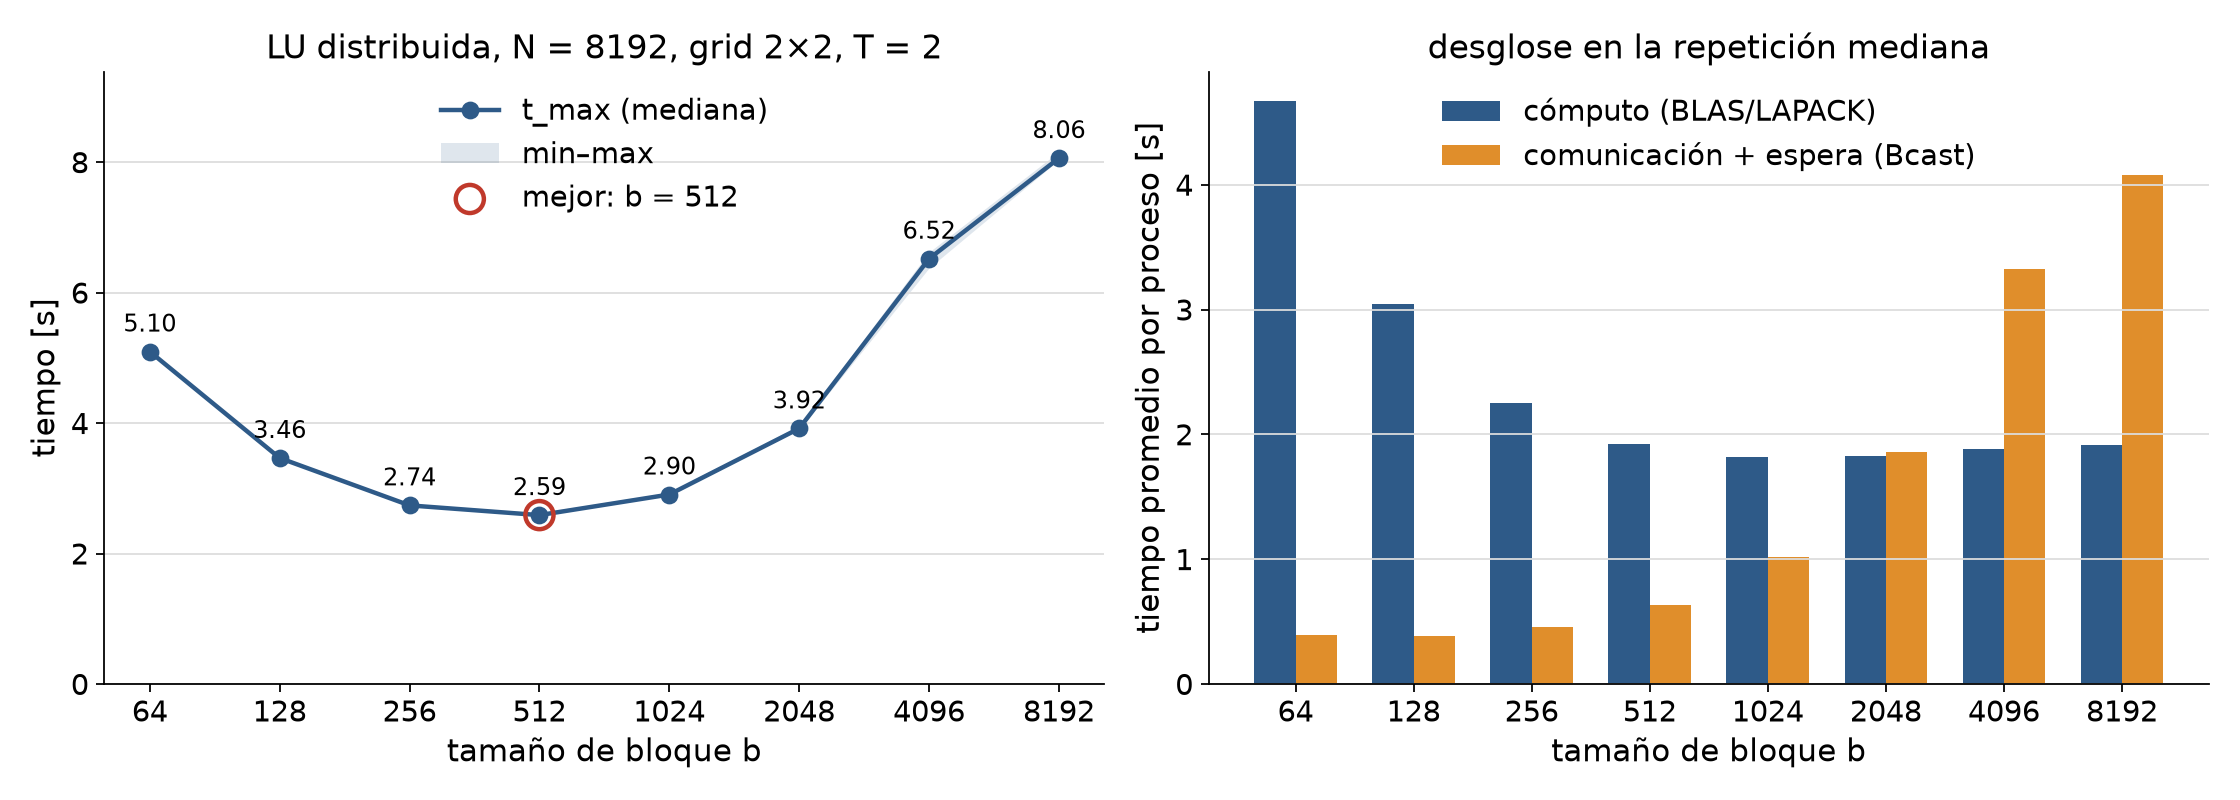
\includegraphics[width=240mm,height=155mm,alt={Barrido en Kraken:
N=8192, grid 2×2 y T=2; los tiempos de comunicación incluyen
espera.}]{figuras/parte_c.png}
\caption{Barrido en Kraken: N=8192, grid 2×2 y T=2; los tiempos de
comunicación incluyen espera.}
\end{figure}

\end{landscape}
\clearpage

\section{(d) Configuraciones 0 a 3: speedup y eficiencia --- 20
puntos}\label{d-configuraciones-0-a-3-speedup-y-eficiencia-20-puntos}

Se usó \(N=8192\) en un nodo \texttt{ventress}, con \(b=512\) y
\(b=1024\). La configuración 0 varía \(T\in\{1,2,4,8\}\) con un proceso;
la 1 usa grids \(1\times2\) y \(2\times1\) con \(T\in\{1,2,4\}\); la 2
usa \(2\times2\) con \(T\in\{1,2\}\); y la 3 compara \(2\times4\) con
\(4\times2\), ambos con \(T=1\). Los datos proceden de
\texttt{results/cluster/config0.csv} a \texttt{config3.csv}.

\subsection{Referencia y métricas}\label{referencia-y-muxe9tricas}

Se define \(T_1(b)\) como la mediana del código distribuido con un
proceso y un thread en el mismo nodo, con igual \(N\) y bloque. Se
obtienen \(T_1(512)=11.208\) s y \(T_1(1024)=10.831\) s. El uso de una
referencia por bloque mide el escalamiento de cada variante, en lugar de
mezclar el efecto del tamaño de bloque con el paralelismo.

\[S(p_r,p_c,T;b)=\frac{T_1(b)}{t_{\max}(p_r,p_c,T;b)},\qquad
E=\frac{S}{p_rp_cT}.\]

Como contraste, si se utiliza una única referencia para comparar ambos
bloques, \(T_1^*=\min_bT_1(b)=10.831\) s, la configuración ganadora con
\(b=512\) obtiene \(S=4.17\) y \(E=52.1\%\). La elección de la
configuración de menor tiempo no cambia.

No se utiliza el tiempo de (a), porque cambia tanto la arquitectura como
\(N\). En grid \(1\times1\) las colectivas no transfieren entre procesos
y su tiempo registrado es cercano a 0.0004 s. Como contraste, las
mediciones seriales del cluster con un thread fueron 11.062 s para
\(b=512\) y 10.507 s para \(b=1024\), diferencias pequeñas respecto a la
referencia distribuida.

\subsection{\texorpdfstring{Resultados con
\(b=512\)}{Resultados con b=512}}\label{resultados-con-b512}

{\def\LTcaptype{none} % do not increment counter
\begin{longtable}[]{@{}lllllll@{}}
\toprule\noalign{}
Config. & Grid & \(T\) & CPUs & Tiempo {[}s{]} & \(S\) & \(E\) \\
\midrule\noalign{}
\endhead
\bottomrule\noalign{}
\endlastfoot
0 & 1×1 & 1 & 1 & 11.208 & 1.00 & 100.0\% \\
0 & 1×1 & 2 & 2 & 6.677 & 1.68 & 83.9\% \\
0 & 1×1 & 4 & 4 & 4.226 & 2.65 & 66.3\% \\
0 & 1×1 & 8 & 8 & 3.058 & 3.66 & 45.8\% \\
1 & 1×2 & 1 & 2 & 6.578 & 1.70 & 85.2\% \\
1 & 1×2 & 2 & 4 & 3.942 & 2.84 & 71.1\% \\
1 & 1×2 & 4 & 8 & 2.620 & 4.28 & 53.5\% \\
1 & 2×1 & 1 & 2 & 6.832 & 1.64 & 82.0\% \\
1 & 2×1 & 2 & 4 & 4.308 & 2.60 & 65.0\% \\
1 & 2×1 & 4 & 8 & 2.983 & 3.76 & 47.0\% \\
2 & 2×2 & 1 & 4 & 4.015 & 2.79 & 69.8\% \\
2 & 2×2 & 2 & 8 & 2.597 & 4.32 & 53.9\% \\
3 & 2×4 & 1 & 8 & 2.670 & 4.20 & 52.5\% \\
3 & 4×2 & 1 & 8 & 2.754 & 4.07 & 50.9\% \\
\end{longtable}
}

\subsection{\texorpdfstring{Resultados con
\(b=1024\)}{Resultados con b=1024}}\label{resultados-con-b1024}

{\def\LTcaptype{none} % do not increment counter
\begin{longtable}[]{@{}lllllll@{}}
\toprule\noalign{}
Config. & Grid & \(T\) & CPUs & Tiempo {[}s{]} & \(S\) & \(E\) \\
\midrule\noalign{}
\endhead
\bottomrule\noalign{}
\endlastfoot
0 & 1×1 & 1 & 1 & 10.831 & 1.00 & 100.0\% \\
0 & 1×1 & 2 & 2 & 6.511 & 1.66 & 83.2\% \\
0 & 1×1 & 4 & 4 & 4.088 & 2.65 & 66.2\% \\
0 & 1×1 & 8 & 8 & 2.971 & 3.65 & 45.6\% \\
1 & 1×2 & 1 & 2 & 6.928 & 1.56 & 78.2\% \\
1 & 1×2 & 2 & 4 & 4.160 & 2.60 & 65.1\% \\
1 & 1×2 & 4 & 8 & 2.754 & 3.93 & 49.2\% \\
1 & 2×1 & 1 & 2 & 7.199 & 1.50 & 75.2\% \\
1 & 2×1 & 2 & 4 & 4.422 & 2.45 & 61.2\% \\
1 & 2×1 & 4 & 8 & 3.079 & 3.52 & 44.0\% \\
2 & 2×2 & 1 & 4 & 4.555 & 2.38 & 59.5\% \\
2 & 2×2 & 2 & 8 & 2.912 & 3.72 & 46.5\% \\
3 & 2×4 & 1 & 8 & 3.167 & 3.42 & 42.8\% \\
3 & 4×2 & 1 & 8 & 3.468 & 3.12 & 39.0\% \\
\end{longtable}
}

Cada tiempo es mediana de tres repeticiones. Los rangos mínimo--máximo
se incluyen en el anexo. La eficiencia se expresa en porcentaje y
considera todas las CPUs, incluidos los threads por proceso.

La configuración con menor mediana es \textbf{configuración 2, grid
\(2\times2\), \(T=2\), \(b=512\)}, con 2.597 s, speedup 4.32 y
eficiencia 53.9\%. Le sigue muy cerca \(1\times2\), \(T=4\), con 2.620
s: la diferencia es menor que 1\%, por lo que no se presenta como una
superioridad concluyente ante cualquier variación de carga del cluster.

Para ocho CPUs y \(b=512\), threads puros (\(1\times1,T=8\)) demoran
3.058 s; MPI puro (\(2\times4,T=1\)), 2.670 s; y el híbrido
(\(2\times2,T=2\)), 2.597 s. El híbrido combina menos participantes MPI
con paralelismo BLAS local. En las repeticiones medianas, MPI puro tiene
cómputo promedio de 1.726 s y comunicación/espera de 0.917 s, mientras
el híbrido presenta 1.932 s y 0.630 s: menor comunicación/espera
compensa un cómputo local algo mayor.

El grid sí afecta los resultados. Para \(b=512,T=4\), \(1\times2\) tarda
2.620 s frente a 2.983 s de \(2\times1\). Con ocho procesos,
\(2\times4\) demora 2.670 s frente a 2.754 s de \(4\times2\). Para
\(b=1024\) la última diferencia aumenta: 3.167 s frente a 3.468 s. En
los datos se favorece sistemáticamente la orientación con más columnas.

El código no es simétrico ante transponer el grid: el panel \(L\) se
resuelve mediante una vista transpuesta y las difusiones del bloque
diagonal se realizan primero por fila y luego por columna. Junto con el
acceso a memoria y las formas de los productos locales, esto ofrece
explicaciones posibles para la asimetría; sin perfilar cada operación
por separado no se asigna una contribución causal exacta a cada una. Por
último, \(b=1024\) es algo mejor en \(1\times1\), mientras \(b=512\)
resulta más rápido en todas las variantes medidas con múltiples procesos
MPI.

\clearpage
\begin{landscape}

\begin{figure}
\centering
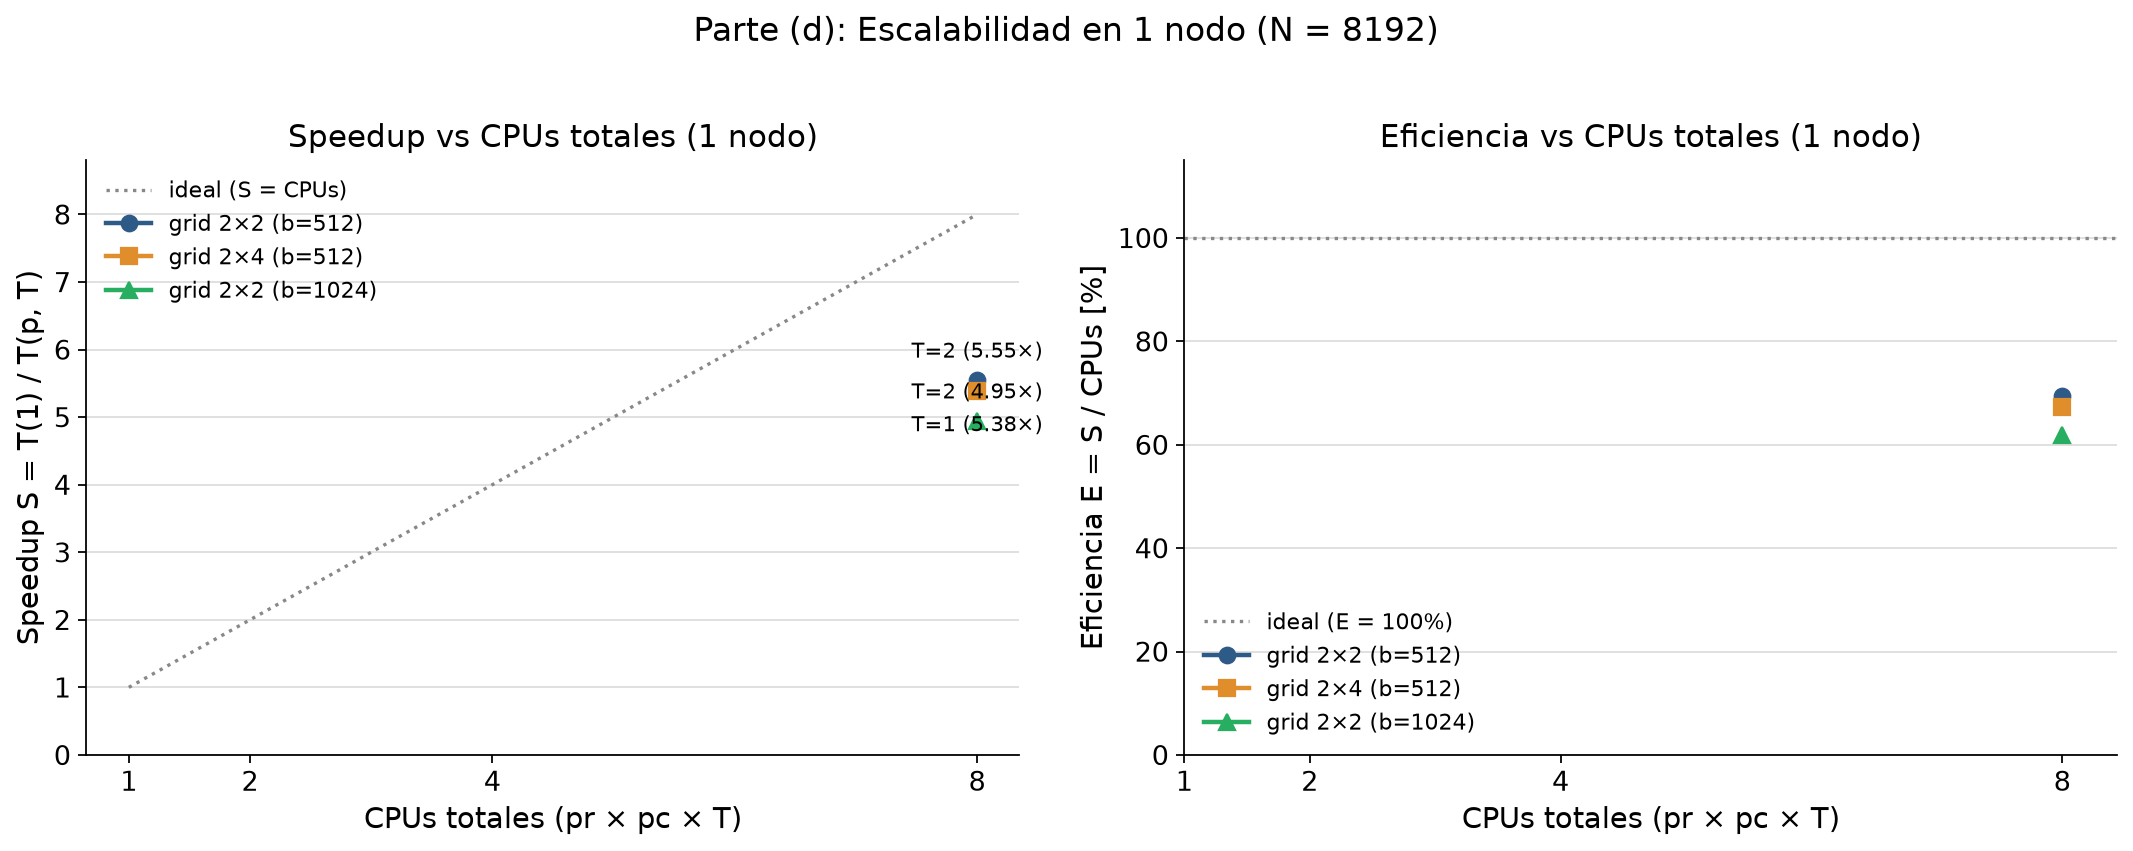
\includegraphics[width=240mm,height=155mm,alt={Speedup y eficiencia en
un nodo para ambos tamaños de bloque. Cada punto utiliza la mediana de
tres repeticiones y una referencia de un proceso y un thread del mismo
bloque.}]{figuras/parte_d.png}
\caption{Speedup y eficiencia en un nodo para ambos tamaños de bloque.
Cada punto utiliza la mediana de tres repeticiones y una referencia de
un proceso y un thread del mismo bloque.}
\end{figure}

\end{landscape}
\clearpage

\section{(e) Configuraciones 4 y 5: dos nodos --- 15
puntos}\label{e-configuraciones-4-y-5-dos-nodos-15-puntos}

Se mantuvo \(N=8192\) y se probaron \(b=512,1024\). La configuración 4
utiliza grid \(2\times4\), \(T=1\) y cuatro procesos por nodo; tiene las
mismas ocho CPUs que la configuración 3 con grid \(2\times4\) en un
nodo. La configuración 5 utiliza grid \(4\times4\), \(T=1\), con ocho
procesos por nodo y 16 CPUs totales. Se utilizan los datos definitivos
de \texttt{config3.csv}, \texttt{config4.csv} y \texttt{config5.csv},
excluyendo las ejecuciones preliminares de \texttt{test\_2nodos.csv}.

{\def\LTcaptype{none} % do not increment counter
\begin{longtable}[]{@{}
  >{\raggedright\arraybackslash}p{(\linewidth - 14\tabcolsep) * \real{0.1250}}
  >{\raggedright\arraybackslash}p{(\linewidth - 14\tabcolsep) * \real{0.1250}}
  >{\raggedright\arraybackslash}p{(\linewidth - 14\tabcolsep) * \real{0.1250}}
  >{\raggedright\arraybackslash}p{(\linewidth - 14\tabcolsep) * \real{0.1250}}
  >{\raggedright\arraybackslash}p{(\linewidth - 14\tabcolsep) * \real{0.1250}}
  >{\raggedright\arraybackslash}p{(\linewidth - 14\tabcolsep) * \real{0.1250}}
  >{\raggedright\arraybackslash}p{(\linewidth - 14\tabcolsep) * \real{0.1250}}
  >{\raggedright\arraybackslash}p{(\linewidth - 14\tabcolsep) * \real{0.1250}}@{}}
\toprule\noalign{}
\begin{minipage}[b]{\linewidth}\raggedright
\(b\)
\end{minipage} & \begin{minipage}[b]{\linewidth}\raggedright
Config.
\end{minipage} & \begin{minipage}[b]{\linewidth}\raggedright
Grid
\end{minipage} & \begin{minipage}[b]{\linewidth}\raggedright
Nodos
\end{minipage} & \begin{minipage}[b]{\linewidth}\raggedright
CPUs
\end{minipage} & \begin{minipage}[b]{\linewidth}\raggedright
Tiempo {[}s{]}
\end{minipage} & \begin{minipage}[b]{\linewidth}\raggedright
\(\bar t_c\) {[}s{]}
\end{minipage} & \begin{minipage}[b]{\linewidth}\raggedright
\(\bar t_m\) {[}s{]}
\end{minipage} \\
\midrule\noalign{}
\endhead
\bottomrule\noalign{}
\endlastfoot
512 & 3 & 2×4 & 1 & 8 & 2.670 & 1.726 & 0.917 \\
512 & 4 & 2×4 & 2 & 8 & 5.668 & 1.858 & 3.754 \\
512 & 5 & 4×4 & 2 & 16 & 4.521 & 0.998 & 3.426 \\
1024 & 3 & 2×4 & 1 & 8 & 3.167 & 1.606 & 1.480 \\
1024 & 4 & 2×4 & 2 & 8 & 6.241 & 1.787 & 4.253 \\
1024 & 5 & 4×4 & 2 & 16 & 5.526 & 0.956 & 4.137 \\
\end{longtable}
}

Con \(b=512\), pasar de configuración 3 a 4 aumenta el tiempo de 2.670 s
a 5.668 s, un factor 2.12. El cómputo promedio pasa de 1.726 s a 1.858
s, mientras comunicación y espera crecen de 0.917 s a 3.754 s,
aproximadamente 4.1 veces. Con \(b=1024\), el tiempo total aumenta de
3.167 s a 6.241 s. Así, distribuir las mismas ocho CPUs en dos nodos
perjudica este problema.

En configuración 4, ranks 0--3 están en \texttt{ventress} y 4--7 en
\texttt{yodaxico}: las filas del grid se comunican dentro del nodo y las
columnas cruzan la red. La latencia \(\alpha\) penaliza cada mensaje y
\(\beta=8/B\) es el costo por palabra float64 para ancho de banda \(B\)
bytes/s. Frente a memoria compartida, mayor latencia y menor ancho de
banda inter-nodo penalizan respectivamente muchas colectivas y paneles
grandes. El aumento de \(t_m\) es consistente con esos efectos, sin
permitir estimarlos por separado. Se distingue además la espera por
diferencias de ejecución local.

\subsection{Desglose de las ejecuciones de dos
nodos}\label{desglose-de-las-ejecuciones-de-dos-nodos}

{\def\LTcaptype{none} % do not increment counter
\begin{longtable}[]{@{}llllll@{}}
\toprule\noalign{}
\(b\) & Config. & Nodo & Ranks & \(\bar t_c\) {[}s{]} & \(\bar t_m\)
{[}s{]} \\
\midrule\noalign{}
\endhead
\bottomrule\noalign{}
\endlastfoot
512 & 4 & ventress & 0--3 & 1.516 & 4.069 \\
512 & 4 & yodaxico & 4--7 & 2.200 & 3.438 \\
512 & 5 & ventress & 0--7 & 0.786 & 3.597 \\
512 & 5 & yodaxico & 8--15 & 1.210 & 3.256 \\
1024 & 4 & ventress & 0--3 & 1.366 & 4.546 \\
1024 & 4 & yodaxico & 4--7 & 2.207 & 3.960 \\
1024 & 5 & ventress & 0--7 & 0.664 & 4.225 \\
1024 & 5 & yodaxico & 8--15 & 1.247 & 4.050 \\
\end{longtable}
}

En configuración 4 con \(b=512\), \texttt{yodaxico} registra 2.200 s de
cómputo promedio frente a 1.516 s de \texttt{ventress}. A su vez,
\texttt{ventress} acumula más espera/comunicación: 4.069 s frente a
3.438 s. Esto es compatible con procesos rápidos esperando a procesos
más lentos. La comparación por host también incluye diferencias de
trabajo entre filas del grid. Una prueba serial previa del grupo
(\(N=2048,b=256,T=1\)) registró 0.224 s en \texttt{ventress} y 0.323 s
en \texttt{yodaxico}, respaldando una posible contribución del hardware.
Sin microbenchmarks, no se separan exactamente red, desbalance y espera.

La configuración 5 reduce el cómputo promedio a 0.998 s para \(b=512\) y
baja el tiempo total a 4.521 s. Es 1.25 veces más rápida que
configuración 4 con el doble de CPUs, lo que equivale a una eficiencia
incremental de aproximadamente 62.7\%. Sin embargo, sigue siendo más
lenta que las ocho CPUs de un solo nodo. Comunicación y espera
representan aproximadamente 77\% de \(\bar t_c+\bar t_m\) en
configuración 5 con \(b=512\); para \(b=1024\) alcanzan 81\%. El aumento
de procesos no compensa los costos de coordinación para este tamaño de
matriz.

\clearpage
\begin{landscape}

\begin{figure}
\centering
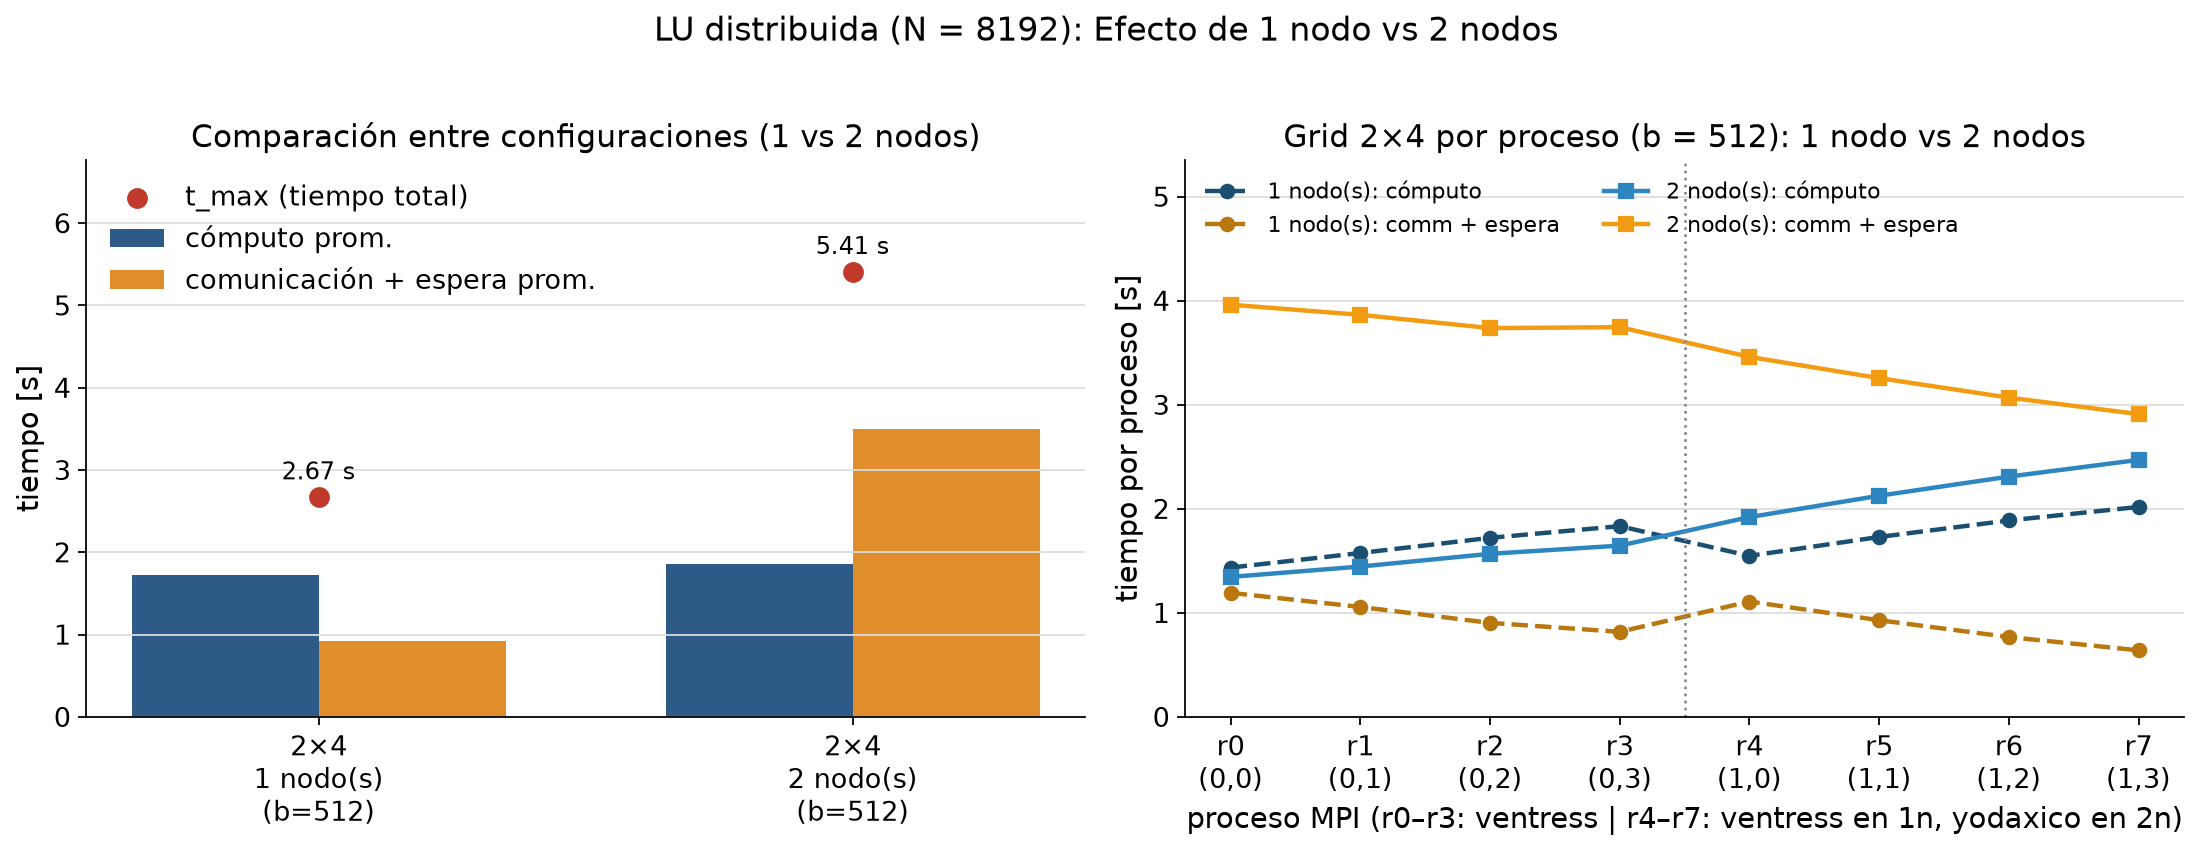
\includegraphics[width=240mm,height=155mm,alt={Comparación de uno y dos
nodos y desglose por proceso. Las barras y curvas de comunicación
incluyen espera.}]{figuras/parte_e.png}
\caption{Comparación de uno y dos nodos y desglose por proceso. Las
barras y curvas de comunicación incluyen espera.}
\end{figure}

\end{landscape}
\clearpage

\section{(f) Efecto del bloque sobre cada proceso --- 15
puntos}\label{f-efecto-del-bloque-sobre-cada-proceso-15-puntos}

Se comparan \(b=N/2=4096\) y \(b=N/16=512\) con \(N=8192\), grid
\(2\times2\), \(T=2\) y un nodo \texttt{ventress}. Se reutilizan las
mediciones de \texttt{parte\_c.csv}: el inciso exige el grid y los dos
bloques, sin fijar un valor distinto de \(T\). Para cada bloque se
selecciona la ejecución de tiempo mediano y se presentan los cuatro
procesos de esa misma ejecución.

{\def\LTcaptype{none} % do not increment counter
\begin{longtable}[]{@{}
  >{\raggedright\arraybackslash}p{(\linewidth - 12\tabcolsep) * \real{0.1429}}
  >{\raggedright\arraybackslash}p{(\linewidth - 12\tabcolsep) * \real{0.1429}}
  >{\raggedright\arraybackslash}p{(\linewidth - 12\tabcolsep) * \real{0.1429}}
  >{\raggedright\arraybackslash}p{(\linewidth - 12\tabcolsep) * \real{0.1429}}
  >{\raggedright\arraybackslash}p{(\linewidth - 12\tabcolsep) * \real{0.1429}}
  >{\raggedright\arraybackslash}p{(\linewidth - 12\tabcolsep) * \real{0.1429}}
  >{\raggedright\arraybackslash}p{(\linewidth - 12\tabcolsep) * \real{0.1429}}@{}}
\toprule\noalign{}
\begin{minipage}[b]{\linewidth}\raggedright
\(b\)
\end{minipage} & \begin{minipage}[b]{\linewidth}\raggedright
Rank
\end{minipage} & \begin{minipage}[b]{\linewidth}\raggedright
Coordenadas
\end{minipage} & \begin{minipage}[b]{\linewidth}\raggedright
\(t_c\) {[}s{]}
\end{minipage} & \begin{minipage}[b]{\linewidth}\raggedright
\(t_m\) {[}s{]}
\end{minipage} & \begin{minipage}[b]{\linewidth}\raggedright
\(t_{wall}\) {[}s{]}
\end{minipage} & \begin{minipage}[b]{\linewidth}\raggedright
\(t_{\max}\) {[}s{]}
\end{minipage} \\
\midrule\noalign{}
\endhead
\bottomrule\noalign{}
\endlastfoot
4096 & 0 & (0,0) & 1.313 & 0.114 & 1.427 & 6.520 \\
4096 & 1 & (0,1) & 1.623 & 4.843 & 6.519 & 6.520 \\
4096 & 2 & (1,0) & 1.273 & 5.138 & 6.467 & 6.520 \\
4096 & 3 & (1,1) & 3.316 & 3.202 & 6.520 & 6.520 \\
512 & 0 & (0,0) & 1.774 & 0.767 & 2.569 & 2.589 \\
512 & 1 & (0,1) & 1.927 & 0.629 & 2.589 & 2.589 \\
512 & 2 & (1,0) & 1.880 & 0.675 & 2.587 & 2.589 \\
512 & 3 & (1,1) & 2.114 & 0.449 & 2.589 & 2.589 \\
\end{longtable}
}

Con \(b=4096\) hay solo cuatro bloques globales, uno por proceso. En el
primer paso, rank 0 factoriza \(A_{00}\); ranks 1 y 2 calculan
\(U_{01}\) y \(L_{10}\); rank 3 actualiza \(A_{11}\) y luego factoriza
ese bloque en el siguiente paso. Esto concentra trabajo y dependencias
en rank 3, cuyo cómputo es 3.316 s, frente a 1.273--1.623 s de los otros
procesos.

Ranks 1 y 2 acumulan 4.843 s y 5.138 s en \texttt{Bcast}: gran parte
corresponde a espera por el progreso de otros procesos, no a mayor
cantidad de datos propios que transferir. Rank 0 termina su intervalo
local en 1.427 s porque ya no tiene actualizaciones pendientes; no
existe una barrera final dentro del cronómetro. El tiempo del job sigue
siendo 6.520 s, máximo de los procesos.

Con \(b=512\) hay 256 bloques globales y 64 bloques locales por proceso.
Los 16 pasos reparten mejor las actualizaciones: el cómputo varía entre
1.774 s y 2.114 s y la comunicación/espera entre 0.449 s y 0.767 s.
Aunque hay más llamadas colectivas, disminuye el desbalance y el tiempo
global baja a 2.589 s, aproximadamente \textbf{2.52 veces más rápido}.
Esta comparación muestra por qué contar solo mensajes no basta para
elegir \(b\).

\clearpage
\begin{landscape}

\begin{figure}
\centering
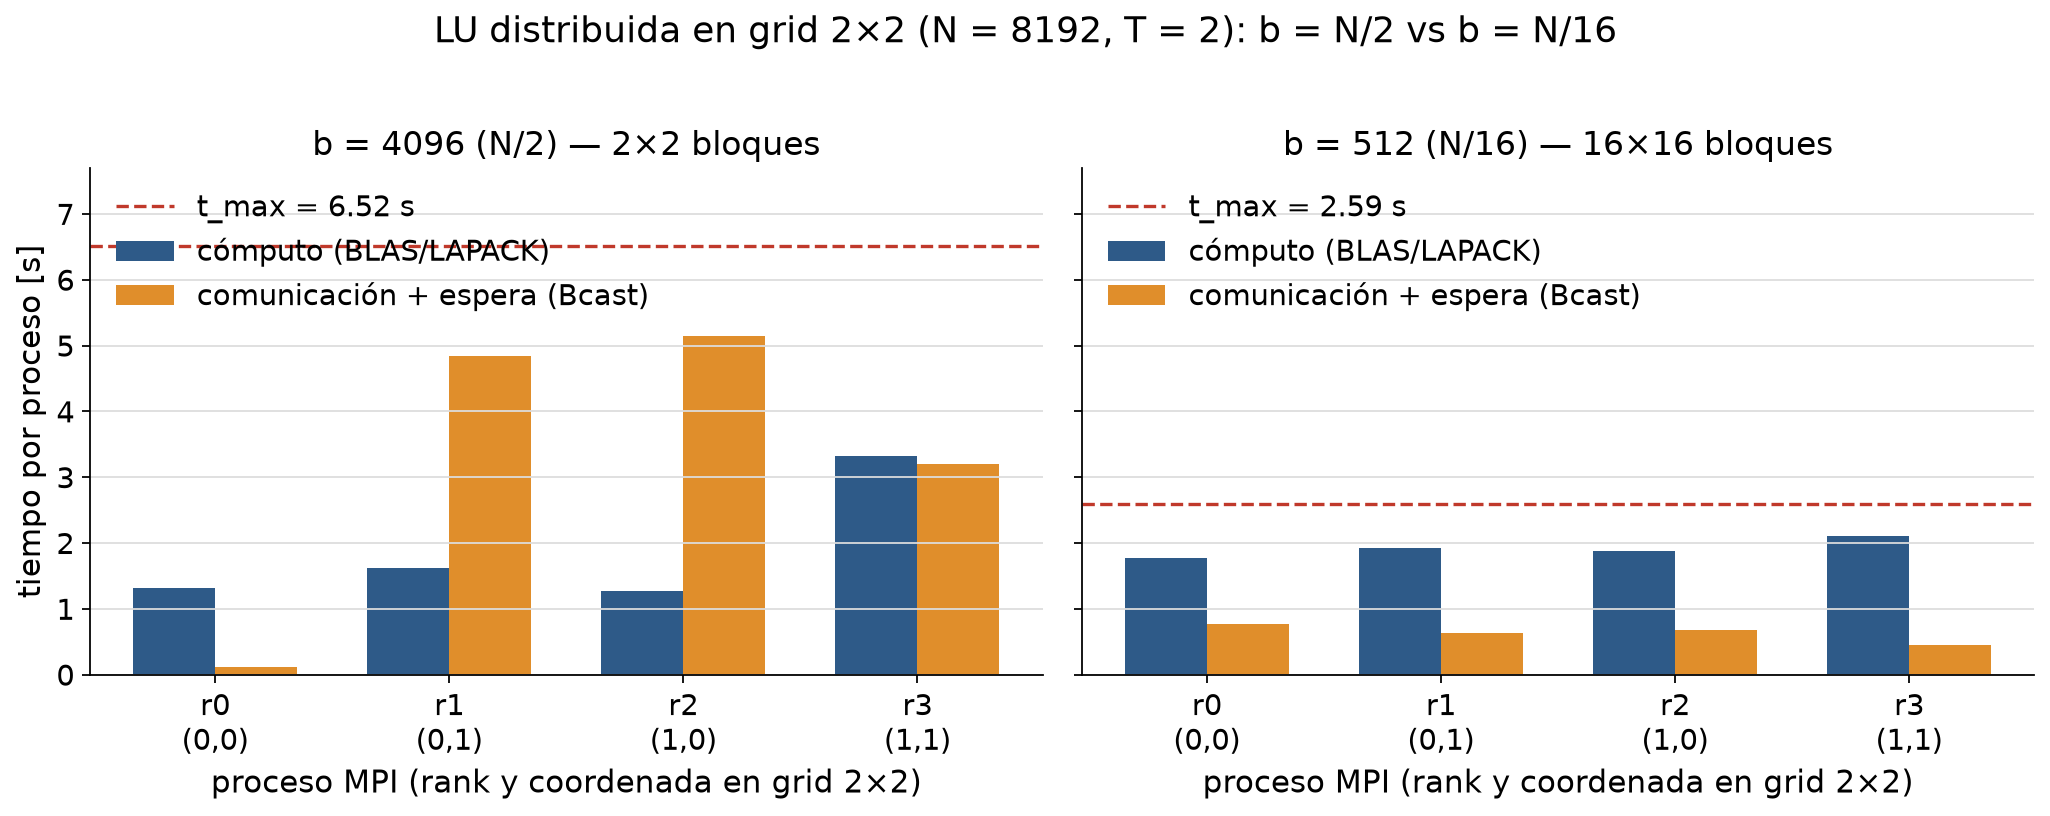
\includegraphics[width=240mm,height=155mm,alt={Tiempos por proceso para
b=N/2 y b=N/16: misma configuración 2×2, N=8192, T=2. Se muestran las
respectivas repeticiones medianas.}]{figuras/parte_f.png}
\caption{Tiempos por proceso para b=N/2 y b=N/16: misma configuración
2×2, N=8192, T=2. Se muestran las respectivas repeticiones medianas.}
\end{figure}

\end{landscape}
\clearpage

\section{(g) Modelo de costo --- 10
puntos}\label{g-modelo-de-costo-10-puntos}

\subsection{Parámetros y costo por
paso}\label{paruxe1metros-y-costo-por-paso}

Sea \(\alpha\) la latencia efectiva por etapa de comunicación {[}s{]},
\(\beta\) el tiempo por palabra float64 {[}s/palabra{]} y \(\gamma\) el
tiempo por flop de un proceso con \(T\) threads {[}s/flop{]}. Se supone
primero hardware homogéneo, bloques repartidos aproximadamente por igual
y un mismo costo efectivo para las primitivas locales. Esta última es
una simplificación: GETRF, TRSM y GEMM tienen eficiencias distintas y
dependen del tamaño.

Para representar una difusión en árbol se define \(h(1)=0\) y
\(h(P)=\lceil\log_2P\rceil\) para \(P>1\), con
\(C_{Bcast}(P,w)\approx h(P)(\alpha+\beta w)\). Es un modelo
orientativo; MPI puede elegir otros algoritmos según el mensaje y el
comunicador. Escribimos \(h_r=h(p_r)\) y \(h_c=h(p_c)\).

En el paso \(k\) queda una submatriz de dimensión \(m_k=N-(k+1)b\). Un
modelo de etapas para su camino crítico es

\[C_k\approx\gamma\left[\frac23b^3+b^2m_k\left(\frac1{p_r}+\frac1{p_c}\right)+\frac{2bm_k^2}{p_rp_c}\right].\]

El primer término corresponde a la factorización de un único bloque
diagonal. Los dos términos de paneles describen el trabajo sobre una
fila y una columna del grid. Se suman como aproximación conservadora: el
dueño de la diagonal participa en ambos, aunque otros procesos pueden
resolver paneles simultáneamente. El último término representa la
actualización distribuida. El tiempo real depende del solapamiento entre
procesos, las llegadas a las colectivas y el desequilibrio discreto de
bloques.

Las difusiones diagonales y de paneles aportan aproximadamente

\[M_k\approx 2\alpha(h_c+h_r)+\beta\left[b^2(h_c+h_r)+bm_k\left(\frac{h_c}{p_r}+\frac{h_r}{p_c}\right)\right].\]

Aquí el panel \(L\), de tamaño aproximado \(bm_k/p_r\), se difunde en
filas de \(p_c\) procesos; el panel \(U\), de tamaño \(bm_k/p_c\), en
columnas de \(p_r\) procesos. Las distintas filas pueden difundir a la
vez: no se multiplica su costo de camino crítico por el número de filas.
En el último paso los paneles están vacíos; conservar sus términos de
latencia es una simplificación de orden menor, y en comunicadores de un
proceso el costo de red se anula por \(h(1)=0\).

\subsection{Suma sobre los pasos}\label{suma-sobre-los-pasos}

Para \(n_b=N/b\),

\[\sum_km_k=\frac{N^2/b-N}{2},\qquad
\sum_km_k^2=\frac{N^3}{3b}-\frac{N^2}{2}+\frac{Nb}{6}.\]

Al sumar se obtiene el modelo de cómputo

\[C\approx\gamma\left[\frac23Nb^2+\frac{N^2b-Nb^2}{2}\left(\frac1{p_r}+\frac1{p_c}\right)+\frac{\frac23N^3-N^2b+\frac13Nb^2}{p_rp_c}\right],\]

y el de comunicación

\[M\approx 2\frac{N}{b}\alpha(h_c+h_r)+\beta\left[Nb(h_c+h_r)+\frac{N^2-Nb}{2}\left(\frac{h_c}{p_r}+\frac{h_r}{p_c}\right)\right].\]

Por tanto, \(t_{modelo}\approx C+M\), al que en una ejecución real se
agregan efectos de desbalance, memoria y administración no capturados
por el reparto continuo. Las fórmulas preservan los términos de borde:
para \(p_r=p_c=1\) se obtiene \(M=0\) y \(C=\gamma(2N^3/3)\),
consistente con que el conteo dominante serial no depende del bloqueo.
Para \(b=N\) se anulan paneles y actualización.

Para identificar la dependencia en \(b\) sin perder términos del mismo
orden, se pueden reagrupar las expresiones anteriores. Definiendo

\[a_p=\frac1{2p_r}+\frac1{2p_c}-\frac1{p_rp_c},\qquad
 d_p=\frac23-\frac1{2p_r}-\frac1{2p_c}+\frac1{3p_rp_c},\]

\[H=h_c+h_r,\qquad K=\frac{h_c}{p_r}+\frac{h_r}{p_c},\]

resulta

\[C\approx\gamma\left[\frac{2N^3}{3p_rp_c}+a_pN^2b+d_pNb^2\right],\]
\[M\approx\frac{2NH\alpha}{b}+\beta\left[\frac{N^2K}{2}+Nb\left(H-\frac K2\right)\right].\]

Los coeficientes \(a_p,d_p\) son no negativos para grids con dimensiones
enteras positivas y se anulan en \(1\times1\). Esta forma evita sumar
correcciones positivas y omitir otras del mismo orden. En un grid
\(2\times2\), \(a_p=d_p=1/4\) y, con el árbol adoptado, \(H=2,K=1\).

Si \(\gamma\) se mantiene constante y se trata \(b\) como continuo, un
óptimo interior satisface

\[\left[\gamma(a_pN+2d_pb)+\beta\left(H-\frac K2\right)\right]b^2=2H\alpha.\]

La ecuación expresa el equilibrio entre el costo creciente de
diagonal/paneles y la latencia decreciente con \(b\). Las expresiones
reagrupadas se contrastaron con las sumas por paso en 49 combinaciones
de parámetros, mediante aritmética racional exacta; el registro está en
\texttt{informe/verificacion/modelo.json}. Luego se deben considerar
solo bloques admisibles que dividan a \(N\). En las mediciones también
cambia la eficiencia BLAS con \(b\), por lo que la ecuación sin
calibración no determina por sí sola el óptimo observado.

Cuando hay pocos bloques por proceso, el reparto continuo \(m_k/p_r\) y
\(m_k/p_c\) es insuficiente. Una aproximación más conservadora utiliza
\(b\lceil(m_k/b)/p_r\rceil\) y \(b\lceil(m_k/b)/p_c\rceil\) para las
dimensiones locales máximas. Esta cuantización explica la pérdida de
paralelismo observada en (f).

\subsection{Óptimo de bloque y cuellos de
botella}\label{uxf3ptimo-de-bloque-y-cuellos-de-botella}

Al disminuir \(b\), crece el número de pasos y el término de latencia
proporcional a \(N/b\). Además, el costo efectivo \(\gamma\) puede
aumentar porque los productos de dimensión interna pequeña aprovechan
peor BLAS y la memoria. En (c), el aumento de cómputo de 1.820 s con
\(b=1024\) a 4.672 s con \(b=64\) muestra que el costo por flop no es
constante en la práctica. El tiempo de comunicación/espera de unos 0.39
s con bloques pequeños no permite, por sí solo, estimar una latencia
pura.

Al aumentar \(b\), crecen el trabajo diagonal serializado (\(Nb^2\)), el
trabajo de paneles con paralelismo restringido (\(N^2b\)) y el volumen
diagonal (\(Nb\)). También disminuye el número de bloques disponibles
para equilibrar el trabajo. El mínimo medido en \(b=512\) es compatible
con un equilibrio entre estas tendencias; el modelo sin parámetros
calibrados no predice numéricamente que el mínimo deba ser exactamente
512.

Los cuellos de botella observados dependen del régimen:

\begin{itemize}
\tightlist
\item
  \textbf{Un nodo y bloque intermedio:} en configuración 2,
  \(b=512,T=2\), el cómputo promedio es 1.932 s y comunicación/espera
  0.630 s, aproximadamente 75\% y 25\% de su suma. Predomina el cómputo
  local, aunque reducir comunicación y desbalance sigue siendo
  relevante.
\item
  \textbf{Bloque grande:} con \(b=4096\) en (f), pocos procesos
  sostienen el camino crítico y otros esperan en las colectivas. La
  restricción principal es el paralelismo insuficiente y la dependencia
  entre etapas, no una transferencia de red demostrada como dominante.
\item
  \textbf{Dos nodos:} en configuración 4 con \(b=512\),
  comunicación/espera promedio alcanza 3.754 s frente a 1.858 s de
  cómputo. La coordinación entre nodos, junto con las diferencias de
  ejecución local, domina el desglose medido. Con 16 CPUs la
  configuración 5 reduce el cómputo, pero la comunicación/espera sigue
  en 3.426 s.
\end{itemize}

Para modelar los dos nodos con mayor fidelidad se necesitarían
parámetros distintos de comunicación intra/inter nodo, costos locales
por host y por primitiva, y medidas separadas de transferencia y espera.
Los CSV disponibles permiten identificar el régimen observado, pero no
ajustar de manera única \(\alpha,\beta,\gamma\).

\section{Conclusiones}\label{conclusiones}

Para la ejecución serial personal se seleccionó \(b=1024\); para el
cluster distribuido, \(b=512\). La menor mediana de las configuraciones
comparadas fue 2.597 s con grid \(2\times2\), dos threads por proceso y
un nodo, muy cercana a 2.620 s de \(1\times2\) con cuatro threads. Los
datos favorecen bloques que permitan repartir suficientes
actualizaciones y una combinación moderada de procesos e hilos. Para
\(N=8192\), repartir el trabajo en dos nodos no mejoró los tiempos de un
nodo. La interpretación depende de distinguir transferencia, espera y
cómputo, y de declarar la configuración exacta de cada medición.

\section{Declaración de uso de IA}\label{declaraciuxf3n-de-uso-de-ia}

Se utilizó ChatGPT/Codex para redactar este informe a partir del código,
apuntes y resultados existentes; contrastar tablas con los CSV; revisar
el modelo de costo; mejorar scripts de verificación y gráficos; ejecutar
comprobaciones locales de correctitud; y preparar los archivos de
compilación y entrega. Los tiempos de rendimiento presentados provienen
de las ejecuciones registradas por el grupo y no fueron reemplazados por
las pruebas locales de auditoría. Las nuevas verificaciones se
identifican por separado y sus resultados se conservaron. Esta
declaración describe la asistencia utilizada para preparar y revisar
este documento.

\section{Anexo: trazabilidad y
reproducción}\label{anexo-trazabilidad-y-reproducciuxf3n}

\subsection{Fuentes del informe}\label{fuentes-del-informe}

El enunciado de referencia es \texttt{docs/tarea03.pdf}. Los resultados
de (a) provienen de \texttt{results/parte\_a\_mac\_jose.csv} y su
archivo de metadatos. Los de (c) y (f) provienen de
\texttt{results/cluster/parte\_c.csv}. Para (d) se usan
\texttt{config0.csv} a \texttt{config3.csv}; para (e),
\texttt{config3.csv} (solo grid \(2\times4\)), \texttt{config4.csv} y
\texttt{config5.csv}. Las mediciones
\texttt{results/parte\_a\_kraken\_T1.csv} permiten contrastar la
referencia serial del cluster. Los apuntes técnicos están en
\texttt{informe/apuntes/}; las afirmaciones sobre verificaciones
históricas se atribuyen a esos registros. Las verificaciones locales
nuevas están documentadas en \texttt{informe/verificacion/};
\texttt{scripts/audit\_results.py} comprueba las 40 grupos de medición
distribuidos, 480 filas por proceso, 21 mediciones seriales y las ocho
tablas numéricas del informe sin modificar los CSV.

Los jobs de las configuraciones definitivas tienen identificadores entre
39644 y 39683, registrados por fila en los CSV. Cada fila representa un
proceso y una repetición. La selección de la repetición mediana conserva
juntos los procesos del mismo job y repetición.

\subsection{Dispersión de las configuraciones (d) y
(e)}\label{dispersiuxf3n-de-las-configuraciones-d-y-e}

Cada fila corresponde a tres repeticiones. El cuerpo del informe
presenta su mediana; esta tabla agrega los extremos observados.

{\def\LTcaptype{none} % do not increment counter
\begin{longtable}[]{@{}lllll@{}}
\toprule\noalign{}
\(b\) & Grid & \(T\) & Mín. {[}s{]} & Máx. {[}s{]} \\
\midrule\noalign{}
\endhead
\bottomrule\noalign{}
\endlastfoot
512 & 1×1 & 1 & 11.192 & 11.326 \\
512 & 1×1 & 2 & 6.602 & 6.748 \\
512 & 1×1 & 4 & 4.197 & 4.233 \\
512 & 1×1 & 8 & 3.057 & 3.113 \\
512 & 1×2 & 1 & 6.522 & 6.592 \\
512 & 1×2 & 2 & 3.927 & 4.088 \\
512 & 1×2 & 4 & 2.606 & 2.648 \\
512 & 2×1 & 1 & 6.812 & 6.932 \\
512 & 2×1 & 2 & 4.293 & 4.414 \\
512 & 2×1 & 4 & 2.965 & 3.005 \\
512 & 2×2 & 1 & 4.004 & 4.140 \\
512 & 2×2 & 2 & 2.592 & 2.617 \\
512 & 2×4 & 1 & 2.668 & 2.736 \\
512 & 4×2 & 1 & 2.738 & 2.808 \\
1024 & 1×1 & 1 & 10.805 & 10.943 \\
1024 & 1×1 & 2 & 6.422 & 6.617 \\
1024 & 1×1 & 4 & 4.054 & 4.286 \\
1024 & 1×1 & 8 & 2.945 & 2.995 \\
1024 & 1×2 & 1 & 6.844 & 7.077 \\
1024 & 1×2 & 2 & 4.124 & 4.234 \\
1024 & 1×2 & 4 & 2.746 & 2.823 \\
1024 & 2×1 & 1 & 7.093 & 7.247 \\
1024 & 2×1 & 2 & 4.413 & 4.521 \\
1024 & 2×1 & 4 & 3.057 & 3.116 \\
1024 & 2×2 & 1 & 4.534 & 4.596 \\
1024 & 2×2 & 2 & 2.899 & 2.935 \\
1024 & 2×4 & 1 & 3.142 & 3.235 \\
1024 & 4×2 & 1 & 3.463 & 3.519 \\
512 & 2×4 (2 nodos) & 1 & 5.631 & 5.726 \\
512 & 4×4 (2 nodos) & 1 & 4.504 & 4.531 \\
1024 & 2×4 (2 nodos) & 1 & 6.216 & 6.278 \\
1024 & 4×4 (2 nodos) & 1 & 5.507 & 5.526 \\
\end{longtable}
}

\subsection{Comandos de reproducción}\label{comandos-de-reproducciuxf3n}

Desde la raíz del repositorio, el entorno y las verificaciones pueden
prepararse con:

\begin{samepage}

\begin{Shaded}
\begin{Highlighting}[]
\ExtensionTok{conda}\NormalTok{ env create }\AttributeTok{{-}f}\NormalTok{ environment.yml}
\ExtensionTok{conda}\NormalTok{ activate tarea3}
\ExtensionTok{python}\NormalTok{ tests/test\_layout.py}
\FunctionTok{bash}\NormalTok{ scripts/test\_distributed.sh}
\ExtensionTok{python}\NormalTok{ scripts/audit\_results.py}
\end{Highlighting}
\end{Shaded}

\end{samepage}

Para regenerar las figuras a partir de los CSV existentes:

\begin{samepage}

\begin{Shaded}
\begin{Highlighting}[]
\ExtensionTok{python}\NormalTok{ scripts/plot\_parte\_a.py }\AttributeTok{{-}{-}tag}\NormalTok{ mac\_jose}
\ExtensionTok{python}\NormalTok{ scripts/plot\_parte\_c.py}
\ExtensionTok{python}\NormalTok{ scripts/plot\_parte\_d.py}
\ExtensionTok{python}\NormalTok{ scripts/plot\_parte\_e.py}
\ExtensionTok{python}\NormalTok{ scripts/plot\_parte\_f.py}
\end{Highlighting}
\end{Shaded}

\end{samepage}

Las figuras (c)--(f) muestran comunicación incluyendo espera. La figura
(f) explicita también los threads BLAS por proceso. Los scripts SLURM y
la descripción del lanzamiento están en \texttt{slurm/}. No es necesario
repetir jobs para compilar el documento.

Con Pandoc y Tectonic disponibles, desde la raíz:

\begin{samepage}

\begin{Shaded}
\begin{Highlighting}[]
\FunctionTok{bash}\NormalTok{ scripts/build\_informe.sh}
\FunctionTok{bash}\NormalTok{ scripts/make\_zip.sh}
\end{Highlighting}
\end{Shaded}

\end{samepage}

El primer comando genera \texttt{informe/informe.tex} e
\texttt{informe/informe.pdf}; el segundo construye el ZIP con los
scripts SLURM, código, pruebas, resultados, fuentes del informe y el
PDF, excluyendo auxiliares y ZIPs anidados. Para Overleaf se incluye un
paquete de fuentes separado con el archivo LaTeX y sus figuras.

\end{document}
